\chapter{Introdução}

Inteligência artificial é um campo da ciência da computação que estuda
``agentes inteligentes'', que de certa forma percebem o ambiente à sua volta
e tomam ações tendo como objetivo maximizar a chance de sucesso de alguma
tarefa específica. Uma utilização muito comum nos dias de hoje é a de
inteligência artificial com o objetivo de criar um agente capaz de competir
com humanos em jogos com alto nível de estratégia, como Xadrez e Go.
Decidimos então estudar inteligência artificial para a realização deste
trabalho com a ideia de modelar um outro jogo de estratégia,
\textbf{Magic: The Gathering}.

\textbf{Magic} foi lançado em 1993, introduzindo o conceito de trading card
game. Com o sucesso do jogo e popularização dos jogos digitais, eventualmente
nasceram versões digitais do jogo para computadores e videogames, e com isso
nasceu a necessidade de agentes que jogassem contra os jogadores. Atualmente
há várias versões digitais de \textbf{Magic}, mas nenhuma tem uma inteligência artificial
boa o suficiente para se provar desafiadora contra jogadores experientes, uma vez
que para cada ação há uma grande quantidade de possibilidades e elementos como
blefe envolvidos. Nossa intenção é entender a complexidade da representação do
jogo e criar uma plataforma para jogar \textbf{Magic} que possibilite a implementação de
um agente de inteligência artificial.

Na próxima seção iremos introduzir alguns conceitos e regras básicas do jogo,
de modo a possibilitar a familiarização do leitor com \textbf{Magic}, facilitando
a compreensão do restante do trabalho.

\section{Conceitos básicos}
Um jogo usual de \textbf{Magic: the Gathering} conta com dois jogadores munidos
de um baralho de 60 cartas cada, ambos começando com 20 pontos de vida, sendo
que o objetivo é reduzir o total de pontos de vida do oponente a 0. Para tanto,
é preciso usar as cartas disponíveis na mão, que podem representar feitiços,
criaturas ou terrenos (existem outros tipos de cartas, mas para nossa implementação
iremos focar nesses três).

\subsection{Cartas}

Nesta seção explicamos a estrutura de uma carta e as diferenças entre os três tipos de carta que utilizamos no projeto. Antes de tudo, convém definir alguns termos utilizados no jogo:

\begin{itemize}
  \item \textbf{Jogar} uma carta é um termo genérico para ``retirar uma carta da sua mão e aplicar seus efeitos no jogo''. Dependendo do tipo de uma carta, quando esta é ``jogada'', será colocada no \textit{campo de batalha} (termo próprio para a mesa de jogo) ou no \textit{cemitério} (termo próprio para a pilha de descarte) do jogador. Uma carta na mesa é chamada \textit{permanente}.
  \item \textbf{Virar} (em inglês, \textit{tap}) uma permanente significa fisicamente dispô-la horizontalmente (normalmente uma carta está na posição vertical). Esta ação representa uma espécie de ação das permenentes. Quando o turno começa, o jogador ativo \textit{desvira} suas permanentes (ou seja, as dispõe em posição vertical), portanto, usualmente, virar uma permanente é um movimento que acontecerá em até uma vez (por permanente) durante cada turno.
\end{itemize}

A seguir, examinaremos a estrutura de uma carta.

\begin{figure}[!ht]
    \centering
    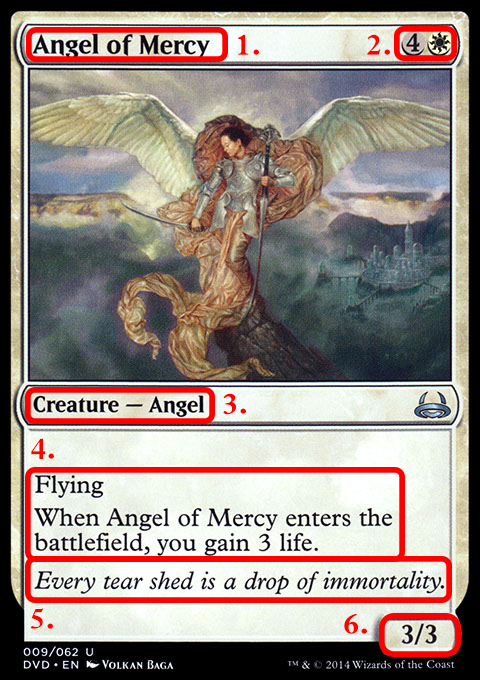
\includegraphics[width=0.65\textwidth]{picstcc/angelnumbers.png}
    \caption{Angel of Mercy e seus principais atributos.}
    \label{cardinfo}
\end{figure}

\begin{enumerate}
  \item \textbf{Nome} da carta.
  \item \textbf{Custo de mana}. ``Mana'' é o recurso necessário em \textbf{Magic} para jogar cartas que não sejam terrenos. Os símbolos da caixa representam a quantidade e tipo de mana necessários para jogar Angel of Mercy.
  $\vcenter{\hbox{
\includegraphics[scale=0.015]{picstcc/4.png}}}$$\vcenter{\hbox{
\includegraphics[scale=0.015]{picstcc/W.png}}}$, então, significa que, para jogar a carta é preciso 4 ``manas'' de qualquer tipo e uma ``mana'' branca, totalizando 5. Mana é geralmente de um dos 5 tipos -- chamados \textit{cores} -- possíveis: Branco ($\vcenter{\hbox{
\includegraphics[scale=0.015]{picstcc/W.png}}}$), Azul, ($\vcenter{\hbox{
\includegraphics[scale=0.015]{picstcc/U.png}}}$), Preto ($\vcenter{\hbox{
\includegraphics[scale=0.015]{picstcc/B.png}}}$), Vermelho ($\vcenter{\hbox{
\includegraphics[scale=0.015]{picstcc/R.png}}}$) e Verde ($\vcenter{\hbox{
\includegraphics[scale=0.015]{picstcc/G.png}}}$). O custo ainda determina a \textit{cor} da própria carta: Angel of Mercy requer apenas mana branca, portanto é uma carta branca.
  \item \textbf{Tipos} de cartas são escritos nesta caixa. Como já mencionado, o tipo de Angel of Mercy é Criatura. Além disso, cartas -- quase sempre criaturas -- também podem ter \textit{subtipos} indicando características da criatura, no caso, um Anjo. Isto é relevante para alguns efeitos do jogo, mas nenhum deles é abordado no projeto.
  \item \textbf{Habilidades} definem os efeitos próprios das cartas. Neste trabalho, usamos apenas criaturas com \textit{habilidades de combate}, características de cada criatura que definem seu comportamento na etapa de combate, e habilidades do tipo ``ao entrar em jogo'', desencadeadas quando a carta se torna uma permanente. \\ No caso, Angel of Mercy tem instâncias dos dois tipos: \textit{Flying} (em portugês, Voar), que limita as interações do oponente durante a etapa de Combate, e sua segunda habilidade, que concede a seu controlador um bônus de 3 pontos de vida. Existem, também, criaturas sem habilidades (porém não existem feitiços sem habilidades). Algumas cartas contêm explicações, em parênteses, de efeitos comuns (como Voar).
  \item \textit{\textbf{Flavor text}} é um texto que ambienta a carta dentro de alguma temática. Pode ser uma fala, um comentário, ou até uma pequena história. \textit{Flavor texts} são escritos em itálico e não influenciam em nada as regras do jogo.
  \item Esta caixa contém os atributos mais importantes das criaturas (e presentes apenas neste tipo de carta): \textbf{poder e resistência}. $X/Y$ representa uma criatura com poder $X$ e resistência $Y$, ou seja, na etapa de combate, esta criatura causa $X$ de dano total e, a qualquer momento, se a criatura tiver uma quantidade $d$ de dano marcado tal que $d \ge Y$, a criatura é destruída.
\end{enumerate}
Os \textbf{terrenos} citados são responsáveis por gerar mana para jogar cartas com custo. Para jogar um terreno, o jogador ativo simplesmente o retira da sua mão e coloca em campo (podendo fazer isso no máximo uma vez por turno). Neste trabalho usamos apenas terrenos com o supertipo \textit{Básico}.\footnote{Geralmente, em \textbf{Magic}, um baralho tem a limitação de 4 cópias de uma mesma carta. Cartas com o supertipo \textit{Básico} não são afetadas por esta limitação.} A cor da mana gerada pelo terreno está ligada a seu subtipo e seu símbolo associado também aparece na carta. Todos os terrenos básicos têm a habilidade ``$\vcenter{\hbox{
\includegraphics[scale=0.015]{picstcc/T.png}}}$: adicione $C$ à sua reserva de mana.'', onde $C \in \left\{ \vcenter{\hbox{
\includegraphics[scale=0.015]{picstcc/W.png}}}, \vcenter{\hbox{
\includegraphics[scale=0.015]{picstcc/U.png}}}, \vcenter{\hbox{
\includegraphics[scale=0.015]{picstcc/B.png}}}, \vcenter{\hbox{
\includegraphics[scale=0.015]{picstcc/R.png}}}, \vcenter{\hbox{
\includegraphics[scale=0.015]{picstcc/G.png}}}\right\}$, não escrita na carta.
\begin{figure}[!h]
  \centering
  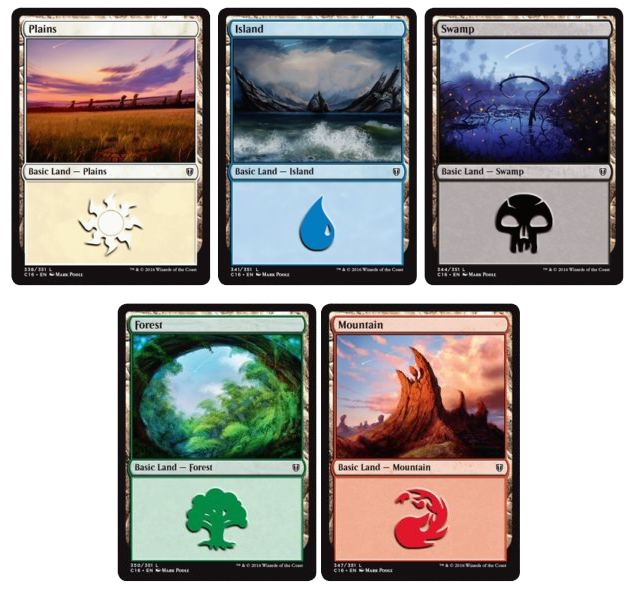
\includegraphics[width=0.7\textwidth]{picstcc/basiclands.png}
  \caption{Os cinco terrenos básicos. Em sentido horário: Planície, Ilha, Pântano, Montanha, Floresta.}
  \label{basiclands}
\end{figure}
\vskip1ex

Assim, a rotina para jogar uma carta com determinado custo é virar o número de terrenos necessários de cada tipo, remover a carta da mão e aplicar seus efeitos (caso seja uma Criatura, é colocada em campo e se torna uma Permanente, caso seja um Feitiço, seus efeitos são aplicados e é colocada no cemitério). No caso de Angel of Mercy, o jogador deve virar 4 terrenos quaisquer e uma Planície para jogá-la. Assim, que o anjo entrar em jogo, seu efeito é desencadeado Apesar de ser possível (e usual) usar mais de uma cor em um baralho, para este trabalho trabalharemos com baralhos de só uma cor.

\begin{figure}[!h]
  \centering
  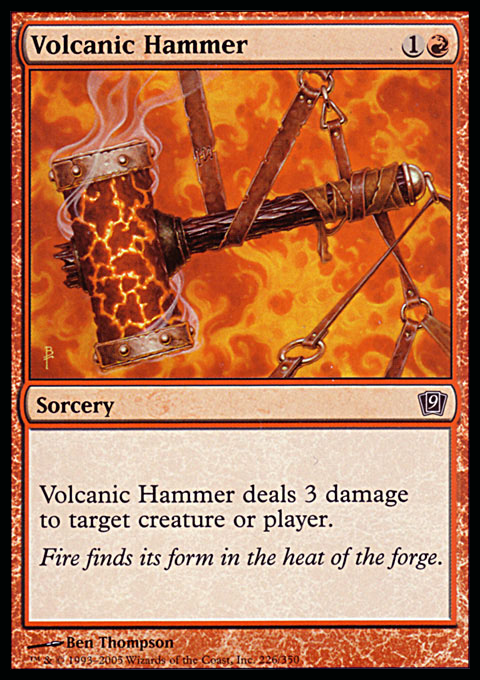
\includegraphics[width=0.4\textwidth]{picstcc/volcanicfull.png}
  \caption{O Feitiço ``Volcanic Hammer'' (Martelo Vulcânico)}
  \label{volcanicsorcery}
\end{figure}

A figura \ref{volcanicsorcery} contém, enfim, um exemplo de Feitiço. A carta possui todas as características de uma carta de Criatura, exceto pelo poder e resistência. Para jogar Volcanic Hammer, além de virar o número de terrenos necesário (ou seja, uma Montanha e um terreno qualquer para pagar o custo de $\vcenter{\hbox{
\includegraphics[scale=0.015]{picstcc/1.png}}} \vcenter{\hbox{
\includegraphics[scale=0.015]{picstcc/R.png}}}$), o jogador ativo deve eleger um \textbf{alvo} para o efeito da carta. O próprio efeito descreve os alvos legais -- no caso, o alvo escolhido pode ser qualquer criatura em campo \textit{ou} qualquer jogador. Alguns efeitos tem seus alvos restritos, por exemplo, a criaturas do oponente ou somente a jogadores.

\vskip1ex

\label{gamestructure}

No começo do jogo é decidido aleatoriamente quem será o jogador inicial,
e então os dois jogadores compram uma mão inicial de sete cartas.
Antes do jogo propriamente dito começar, os jogadores podem optar por tomar uma
ação chamada mulligan, que consiste em rejeitar a mão inicial, embaralhá-la
de volta com o restante dos cards e comprar uma nova mão inicial, com uma carta
a menos. Pode-se então repetir o processo até que cada jogador esteja satisfeito
com a mão inicial ou até o jogador realizar um mulligan com apenas uma carta na
mão (resultando em uma mão de zero cartas, onde não há mais a possibilidade de
realizar mulligan). Uma vez que os dois jogadores tiverem escolhido manter uma
mão inicial, cada jogador que realizou pelo menos um mulligan olha a carta do
topo de seu \textit{deck} (como é chamado o baralho) e decide se quer colocá-la
no fundo.

\vskip1ex

O jogo então começa, com os jogadores alternando entre turnos, onde o
jogador que ``controla o turno'' é chamado de \textit{jogador ativo},
com a seguinte estrutura, simplificada:

\begin{itemize}
    \item\textbf{Início do turno}: Permanentes do jogador ativo são
desviradas. Jogador ativo compra uma carta de seu deck.
    \item\textbf{Primeira Fase Principal}: Jogador ativo pode jogar as
cartas da mão. Termina quando o jogador ativo decide \textit{passar}, o que implica no término da fase atual.
    \item \textbf{Combate}: O combate é a maneira principal de um jogador ganhar o jogo, pois envolve a tentativa de diminuição dos pontos de vida de seu oponente através de ataques de suas criaturas. Será melhor explicado na próxima seção.
    \item \textbf{Segunda Fase Principal}: Igual à primeira Fase Principal.
    \item \textbf{Fase final}: Todas as criaturas tem seu dano marcado revertido para 0. Caso o jogador tenha mais de sete cartas na mão, deve descartar (colocar no \textit{cemitério}) até ter uma mão de sete cartas.
\end{itemize}

A estrutura acima se repete até o jogo terminar, o que acontece
geralmente quando algum jogador chega a 0 pontos de vida,
mas também pode acontecer de outras maneiras como, por exemplo, se o
baralho de um jogador acabar.

\subsection{Exemplo de Fases Principais}

Suponhamos que o jogador ativo tem 5 Planícies desviradas e 20 pontos de vida. Na sua primeira Fase Principal, joga seu Angel of Mercy (virando as 5 planícies para adicionar $\vcenter{\hbox{
\includegraphics[scale=0.015]{picstcc/W.png}}} \vcenter{\hbox{
\includegraphics[scale=0.015]{picstcc/W.png}}}\vcenter{\hbox{
\includegraphics[scale=0.015]{picstcc/W.png}}}\vcenter{\hbox{
\includegraphics[scale=0.015]{picstcc/W.png}}}\vcenter{\hbox{
\includegraphics[scale=0.015]{picstcc/W.png}}}$ à sua reserva de mana), que tem seu efeito desencadeado levando-o a 23 pontos de vida. Decide, então, passar o turno para a fase de Combate. Como não tem nenhuma criatura apta a atacar (melhor explicado na próxima subseção), a fase de Combate termina e começa a segunda Fase Principal. O jogador ativo decide passar a segunda fase principal. No próximo turno, o jogador ativo é trocado, compra uma carta e inicia sua primeira Fase Principal. O (novo) jogador ativo tem duas montanhas e decide jogar Volcanic Hammer alvejando Angel of Mercy (e para fazê-lo, vira as duas montanhas, gerando $\vcenter{\hbox{
\includegraphics[scale=0.015]{picstcc/R.png}}} \vcenter{\hbox{
\includegraphics[scale=0.015]{picstcc/R.png}}}$). Como o anjo tem 3 de resistência e o Feitiço lhe causa 3 dano, a permanente é destruída.

\subsection{Combate}

A fase de Combate é a principal maneira do jogador ativo diminuir o total de vida de seu oponente. Isto é realizado ao \textbf{atacar} com suas criaturas. O jogador defensor, como é chamado o oponente do jogador ativo, tem a chance de \textbf{bloquear} os ataques com as suas próprias criaturas. A maioria dos jogos de \textbf{Magic} termina durante esta fase.

\begin{enumerate}
  \item Jogador ativo \textit{declara atacantes} -- escolhe
quais de suas criaturas irão atacar seu oponente. Uma criatura só pode atacar se 1) estiver \textbf{desvirada} (representada na posição vertical) e 2) não estiver \textit{enjoada} (termo que significa que a criatura entrou em jogo neste turno -- uma criatura só pode atacar a partir do turno seguinte ao turno que entrou no campo de batalha). Uma vez que o jogador decidiu com quais criaturas atacar, deve \textbf{virar} as criaturas declaradas para indicar que estas estão atacando. Se o jogador ativo não tiver criaturas aptas a atacar (ou decidir não atacar com nenhuma), a fase de Combate termina.
    \item O jogador defensor \textit{declara bloqueadores} -- escolhe quais de suas criaturas irão
bloquear as criaturas atacantes. Mais uma vez, apenas criaturas \textbf{desviradas} podem bloquear. Diferentemente das criaturas atacantes, porém, criaturas bloqueadoras \textbf{não} se tornam viradas por executar essa ação. Algumas habilidades restringem como criaturas podem bloquear: uma criatura atacante com Voar só pode ser bloqueada por criaturas com a habilidade Voar ou Alcance (\textit{Reach}).
    \item Caso alguma criatura atacante esteja bloqueada
por mais de uma criatura, o jogador ativo decide, então, a ordem com que o dano será
atribuído a cada criatura bloqueadora.
    \item Por fim, há a atribuição de dano. Cada criatura atacante causa dano igual a seu poder às criaturas que a bloqueiam e, caso, não esteja bloqueada, causa dano igual ao seu poder ao jogador defensor. Cada criatura bloqueadora causa dano igual ao seu poder à criatura que bloqueou.
\end{enumerate}

\subsection{Exemplo de Combate}

Suponhamos que o jogador ativo tenha três criaturas desviradas e não-enjoadas no início da fase de combate e seu oponente tenha duas criaturas desviradas (portanto, aptas a bloquear) e 20 pontos de vida.

\begin{figure}[!h]
  \centering
  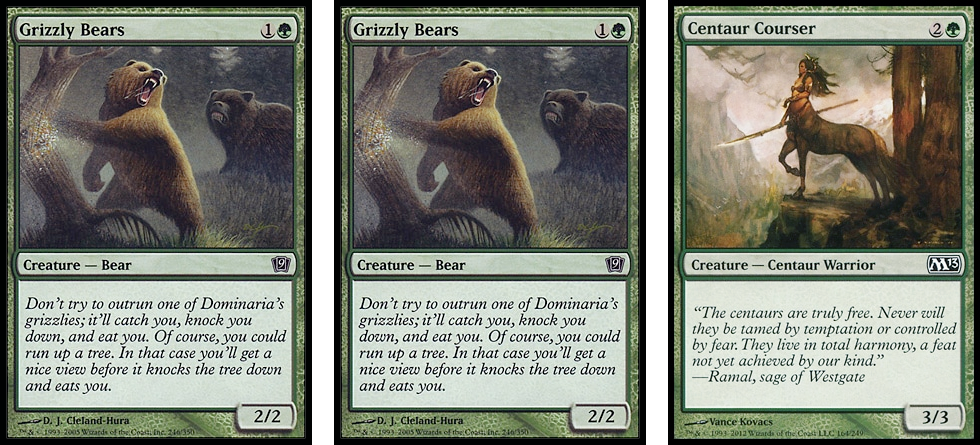
\includegraphics[width=0.75\textwidth]{picstcc/att1.png}
  \caption{Criaturas do jogador ativo: dois ``Grizzly Bears'' (Ursos Cinzentos) em uma ``Centaur Courser'' (Centaura-Caçadora).}
  \label{beginattack}
\end{figure}

\begin{figure}[!h]
  \centering
  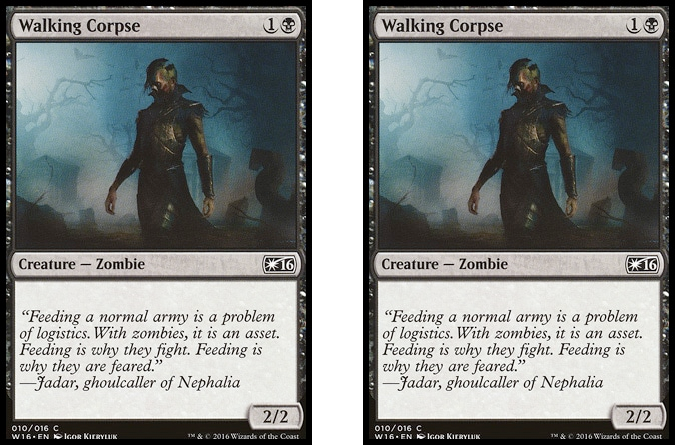
\includegraphics[width=0.55\textwidth]{picstcc/blk1.png}
  \caption{Criaturas do jogador defensor: dois ``Walking Corpse'' (Cadáver Ambulante).}
  \label{beginblock}
\end{figure}

\begin{figure}[!h]
  \centering
  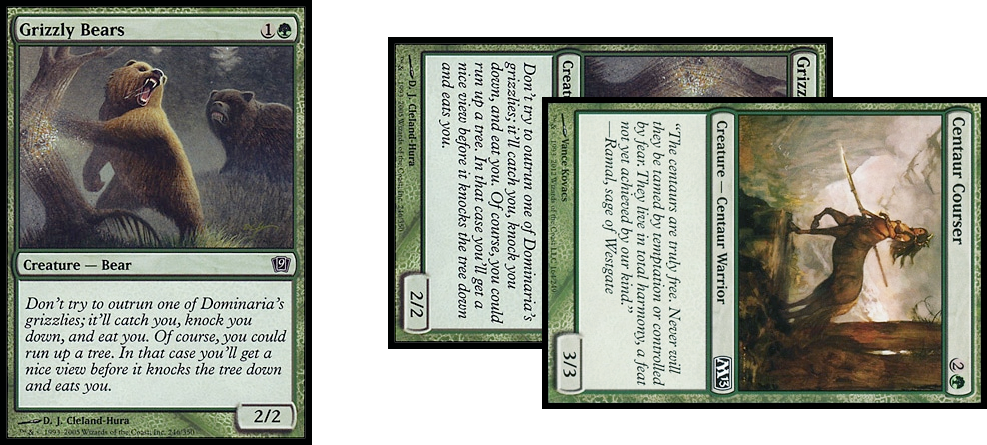
\includegraphics[width=0.7\textwidth]{picstcc/att2.png}
  \caption{Supondo que o jogador ativo decida atacar com Centaur Courser e um Grizzly Bears, deve então virá-los.}
  \label{declaredattackers}
\end{figure}

\begin{figure}[!h]
  \centering
  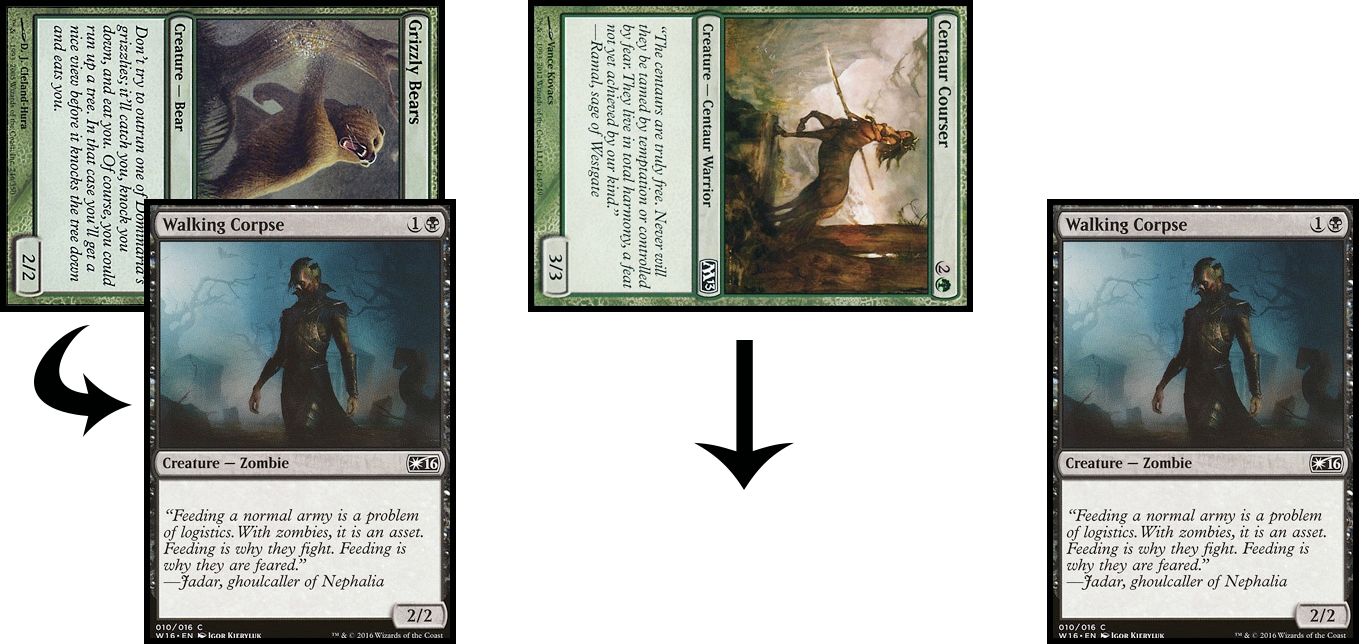
\includegraphics[width=0.7\textwidth]{picstcc/blk2.png}
  \caption{Por fim, o jogador defensor deve declarar quais de suas criaturas bloquearão a ofensiva. Suponhamos, então, que a escolha seja apenas bloquear Grizzly Bears com um Walking Corpse.}
  \label{declaredblockers}
\end{figure}

\begin{figure}
Assim, no final do combate, Grizzly Bears causa 2 de dano a Walking Corpse, que por sua vez também lhe causa 2 de dano. Ambas as criaturas são destruídas. Centaur Courser causa 3 de dano ao jogador defensor. O jogador defensor termina 17 de vida e um Walking Corpse desvirado, enquanto o jogador ativo tem 20 de vida e um Centaur Courser virado.
\end{figure}
